% ══════════════════════════════════════════════════════════════════════════════
%  CHAPTER 5: THERMODYNAMICS AND PRIMORDIAL SOUP
% ══════════════════════════════════════════════════════════════════════════════

\chapter{Thermodynamics and Primordial Soup (Lecture 9-12)}

% ──────────────────────────────────────────────────────────────────────────────
\section{Statistical Distributions}
\subsection{Energy-Momentum Relation}
To calculate the value of various thermodynamic quantities, we need first clarify some basic concepts and notations first for convenience. \\

In below contents, we will use the $E(p)$ notation to represent the energy of a particle with momentum $p$ and mass $m$.
\begin{foundation}
    Recall special relativity, the energy of a particle with mass $m$ and three-momentum $p$ is given by
    \[
        E(\vec{p}) = \sqrt{|\vec{p}|^2c^2 + m^2c^4}.
    \]
    Taken $c = 1$ and $p = |\vec{p}|$, we have $E(p) = \sqrt{p^2 + m^2}$. \\

    In a Non-relativistic limit ($p \ll m$):
    \[
        E(p) = m \sqrt{1 + \frac{p^2}{m^2}} \approx m + \frac{p^2}{2m}.
    \]
    In an Ultra-relativistic limit ($p \gg m$):
    \[
        E(p)  \approx p.
    \]
\end{foundation}

%──────────────────────────────────────────────────────────────────────────────
\bigskip\noindent
\subsection{Chemical Potential}
%Explanation of \mu
\begin{foundation}
    $\mu$ is the chemical potential, which measures the change in internal energy when a particle is added to the system at constant entropy and volume.
\end{foundation}

For ideal gases, $\mu \to 0$, and we will assume $\mu = 0$ in below contents unless otherwise specified.

\begin{remark}
  The chemical potential $\mu$ is typically zero for photons and other massless bosons, while it can be non-zero for massive particles depending on the context (e.g., in a gas of electrons).\\

  while for particles and their own anti-particles, $\mu_+ = -\mu_-$.
\end{remark}

% ────────────────────────────────────────────────────────────────────────────────
%proof of equation
\clearpage
\subsection{Thermal Equilibrium Distributions}
\bigskip\noindent
\begin{foundation}
    For a state with energy $E$, and particle number $N$, 

\end{foundation}

\bigskip\noindent
\begin{theory}
  In thermal equilibrium, the distribution of particle energies follows specific statistical distributions:
  \begin{itemize}
    \item \textbf{Fermi-Dirac distribution} for fermions:
    \[
      f(p) = \frac{1}{e^{(E(p)-\mu)/k_B T} + 1}
    \]
    \item \textbf{Bose-Einstein distribution} for bosons:
    \[
      f(p) = \frac{1}{e^{(E(p)-\mu)/k_B T} - 1}
    \]
    \item \textbf{Maxwell-Boltzmann distribution} for classical particles:
    \[
      f(p) = e^{-(E(p)-\mu)/k_B T}
    \]
  \end{itemize} \\

  In general, the distribution can be written as:
    \[
        f(p) = \frac{1}{e^{(E(p)-\mu)/k_B T} \pm 1},
    \]
  where the $+$ sign is for fermions and the $-$ sign is for bosons.
\end{theory}

\bigskip\noindent
\begin{theory}
    In non-relativistic limit(low temperature $\&$ low density), the Fermi-Dirac and Bose-Einstein distributions reduce to the Maxwell-Boltzmann distribution:
    \[
        e^{(E(p) - \mu)/k_B T} \gg 1 \implies f(p) \approx e^{-(E(p)-\mu)/k_B T}
    \]
\end{theory}

% ──────────────────────────────────────────────────────────────────────────────
\clearpage
\section{Number Density, Energy Density, and Pressure}
\subsection{Spin Degeneracy Factor}
%Explanation of g
In below contents, we define $g$ as Spin degeneracy factor(spin states), which counts the number of internal degrees of freedom (e.g., spin states) for a particle species.
\begin{foundation}
    g
\end{foundation}

\begin{extra}
    The g values for some common particles are:
    \begin{center}
    \begin{tabular}{p{4cm}p{5cm}c}
        \toprule
        Particle & symbol & $g$ \\
        \midrule
        Photon & $g_\gamma$ & 2 \\
        Electron/Positron & $g_e^-, g_e^+$ & 2 \\
        Z boson & $g_Z$ & 3 \\
        Higgs boson & $g_H$ & 1 \\
        \bottomrule
    \end{tabular}
    \end{center}
\end{extra}

%──────────────────────────────────────────────────────────────────────────────
\subsection{Derivation of the 3 equations}
% how the 3 equations are derived
\bigskip\noindent
\begin{foundation}

\end{foundation}

\bigskip\noindent
\begin{theory}
    The number density $n$, energy density $\rho$, and pressure $P$ of some particle i are given by:
    \[
        n_i = \frac{g_i}{(2\pi)^3} \int f_i(p) \, d^3p,
    \]
    \[
        \rho_i = \frac{g_i}{(2\pi)^3} \int E(p) f_i(p) \, d^3p,
    \]
    \[
        P_i = \frac{g_i}{(2\pi)^3} \int \frac{p^2}{3E(p)} f_i(p) \, d^3p
    \]
\end{theory}

%derivation of substitute 3 distributions function into the 3 equations
\bigskip\noindent
\begin{foundation}
    By substituting the Fermi-Dirac, Bose-Einstein, or Maxwell-Boltzmann distribution functions into the above integrals, we can derive explicit expressions for $n_i$, $\rho_i$, and $P_i$ for different particle species under various conditions (e.g., relativistic vs. non-relativistic limits).

    \textbf{(1) Relativistic Fermions ($E \approx p$):}
     \begin{itemize}
        \item Number density: $n_i = \frac{3\zeta(3)}{4\pi^2} g_i T^3$
        \item Energy density: $\rho_i = \frac{7\pi^2}{120} g_i T^4$
        \item Pressure: $P_i = \frac{1}{3}\rho_i$
     \end{itemize} \\

    \textbf{(2) Relativistic Bosons ($E \approx p$):}
     \begin{itemize}
        \item Number density: $n_i = \frac{\zeta(3)}{\pi^2} g_i T^3$
        \item Energy density: $\rho_i = \frac{\pi^2}{30} g_i T^4$
        \item Pressure: $P_i = \frac{1}{3}\rho_i$
     \end{itemize} \\
    \textbf{(3) Non-relativistic Particles ($E \approx m + p^2/2m$):}
     \begin{itemize}
        \item Number density: $n_i = g_i \left( \frac{m_i T}{2\pi} \right)^{3/2} e^{-m_i/T}$
        \item Energy density: $\rho_i = n_i m_i$
        \item Pressure: $P_i = n_i T$
     \end{itemize}
\end{foundation}

\begin{theory}
    Number density, energy density, and pressure for particles with different thermal equilibrium distributions:

    % row is for the 3 distributions, column is for the 3 quantities
    \begin{center}
    {\renewcommand{\arraystretch}{1.8}
    \begin{tabular}{p{3.5cm}|p{2.5cm}|p{2.5cm}|p{3.5cm}}
        \toprule
        & {\small Relativistic Fermions} & {\small Relativistic Bosons} & {\small Non-relativistic Particles (Fermions/ Bosons)} \\
        \midrule
        {\small Number Density $n_i$} & $\frac{3}{4}\frac{\zeta(3)}{\pi^2} g_i T^3$ & $\frac{\zeta(3)}{\pi^2} g_i T^3$ & $g_i \left( \frac{m_i T}{2\pi} \right)^{3/2} e^{-m_i/T}$ \\
        {\small Energy Density $\rho_i$} & $\frac{7}{8}\frac{\pi^2}{30} g_i T^4$ & $\frac{\pi^2}{30} g_i T^4$ & $n_i m_i$ \\
        {\small Pressure $P_i$} & $\frac{1}{3}\rho_i$ & $\frac{1}{3}\rho_i$ & $n_i T$ \\
        \bottomrule
        \end{tabular}
    }
    \end{center}

    where $\zeta(3) \approx 1.202$ is the Riemann zeta function evaluated at 3.
\end{theory}

\bigskip\noindent
We can see once the particles no longer relativistic, the number density and energy density will be exponentially suppressed. \\
It is because in the thermal plasma, the energy of particle are $ E \sim T$, and when $T \ll 2m$, the probability of pair production which require energy $E \geq 2m$ will be very low, thus the number density and energy density will be suppressed.

%\bigskip\noindent
\begin{intuition}
    It also explains why very few positrons exist in the current universe! \\
    In the early universe, $T \gg m_e \approx 0.511\,\mathrm{MeV}$, $e^+e^-$ pairs were abundant. \\
    As the universe cooled below $T \sim m_e$, the number density of positrons (and electrons) dropped exponentially, leaving only a tiny fraction that survived annihilation, which is why we observe so few positrons today.
\end{intuition}

\bigskip\noindent
\begin{theory}
    We can see the relationship between p and $\rho$ for different relativistic limits:
    \[
        P = \begin{cases}
            \frac{1}{3}\rho & ,T \gg m \\
            nT \ll \rho & ,T \ll m
        \end{cases}
    \]

    In fact, it also consistent with the assumption of state parameter of radiation and matter, which are $w = 1/3$ and $w = 0$ when in relativistic and non-relativistic limits respectively.
\end{theory}

\bigskip\noindent
\begin{theory}
    The average particle energy is given by:
    \[
        \langle E \rangle = \frac{\rho_i}{n_i} = \begin{cases}
            \frac{7\pi^4}{180\zeta(3)} T \approx 3.151 T & ,T \gg m \text{ for relativistic fermions} \\
            \frac{\pi^4}{30\zeta(3)} T \approx 2.701 T & ,T \gg m \text{ for relativistic bosons} \\
            m + \frac{3}{2}T & ,T \ll m \text{ for non-relativistic particles}
        \end{cases}
    \]\\

    Thats mean we can have a simplification  of $\langle E \rangle \sim T$ for relativistic particles, as they have same order of magnitude, which is low enough error in astronomy $:)$
\end{theory}















% ──────────────────────────────────────────────────────────────────────────────
\clearpage
\section{Effective Number of Relativistic DOF}
\begin{theory}
    The Friedmann equation shows that the expansion rate of the universe is determined by the total energy density $\rho$:
    \[
        \rho(T) = \sum_i \rho_i(T)
    \]
    where i runs over all particle species in the thermal plasma. \\

    Considering in the the early universe, energy density is dominated by relativistic particles, we can directly sum over the relativistic species, and define the effective number of relativistic degrees of freedom $g_*$ as:
    \[
        \rho(T) = \frac{\pi^2}{30} g_*(T) T^4,
    \]
    where:
    \[
        g_*(T) = \sum_{\text{bosons}} g_i + \frac{7}{8} \sum_{\text{fermions}} g_i
    \]
\end{theory}

\midskip\noindent
\begin{importantnote}
    Note the above equation is only valid in early universe which radiation dominates. When universe cools down and matter dominates, the energy density will be dominated by non-relativistic particles, and above equation will no longer valid. In that case, we need to consider the contribution of non-relativistic particles to the energy density, which is given by $\rho_i = n_i m_i$.
\end{importantnote}

\clearpage
%\bigskip\noindent
\begin{remark}
    $g_*$ is depends on T(i.e. $g_*(T)$), as the sum runs over only relativistic species, with $m_i \ll T$. As the universe cools down, more and more species become non-relativistic and drop out of the sum, thus $g_*$ decreases with time.
\end{remark}

\begin{figure}[htbp]
    \centering
    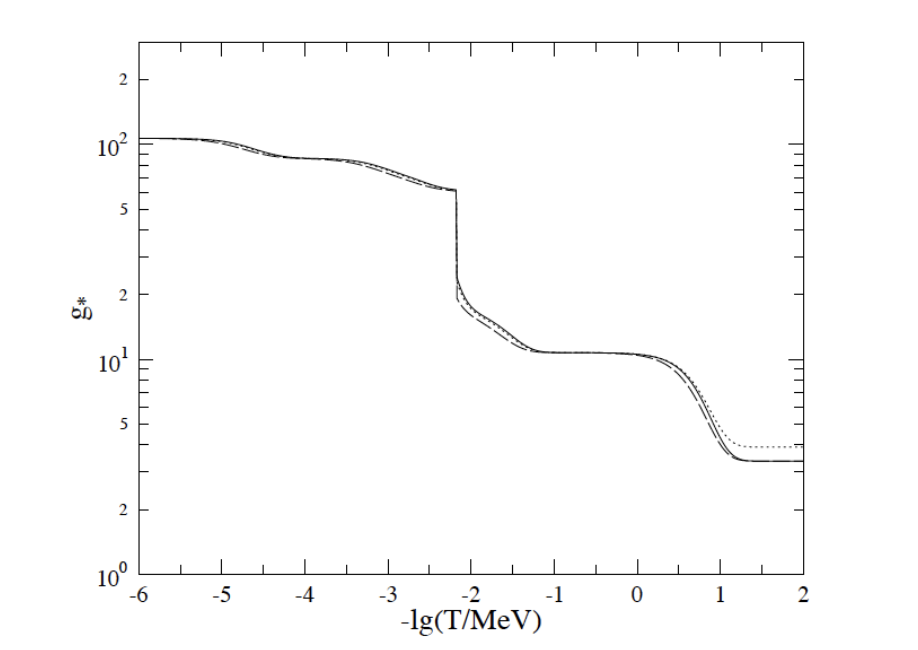
\includegraphics[width=0.8\textwidth]{images/g*_evolution.png}
    \caption{Evolution of $g_*$ with temperature.}
    \label{fig: The evolution of $g_*$ as a function of temperature}
\end{figure}

